%%%%%%%%%%%%%%%%%%%%%%%%%%%%%%%%%%%%%%%%%%%%%%%%%%%%%%%%%%%%%%%%%%%%%%%%%%%%%%%%%%%%%%%%%%%%%%%%%%%


\chapter{Resultados y discusión} \label{chap:AyR}
 En este capítulo, se presentarán y analizarán los resultados obtenidos a partir de los datos recopilados en la investigación. Se examinarán en detalle los hallazgos clave relacionados con la creación del controlador y el funcionamiento del sistema controlado. Además, se discutirán las implicaciones de estos resultados y se expondrán recomendaciones prácticas basadas en los objetivos planteados.

 
\section{Sistema hidropónico DFT}
Para evaluar los resultados de un sistema hidropónico DFT utilizando un controlador basado en lógica difusa se diseñó un experimento para compararlo con un sistema convencional. Se realizaron dos propuestas de sistemas: uno de 8 canales de riego y otro a 2 canales, los cuales se muestran en las figuras \ref{sistema8} y \ref{sistema8_2}. El sistema cuenta con un recipiente de 40 litros donde se encuentra la solución nutritiva donde cada hora se activa la bomba periférica y se realiza el cambio de solución en los canales de riego para oxigenarla.

 \begin{figure}[H]
\centering
         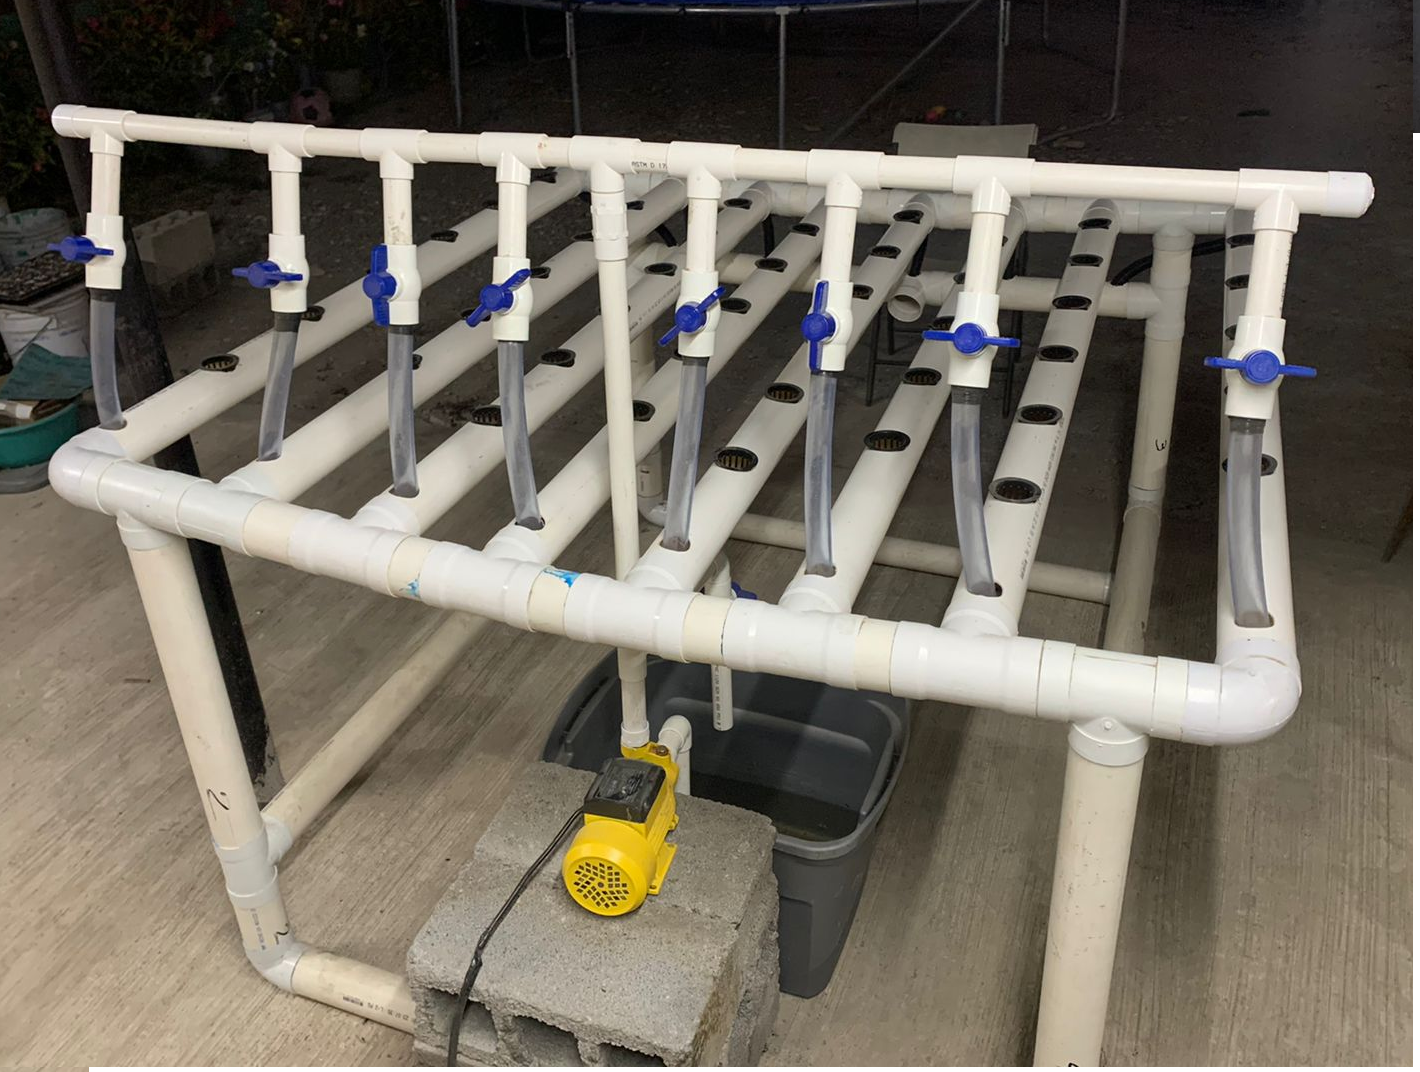
\includegraphics[scale=0.33]{imgs/1.png} \\
    \caption{Sistema hidropónico DFT propuesto de 8 canales. }\label{sistema8}
\end{figure}

 \begin{figure}[H]
\centering
         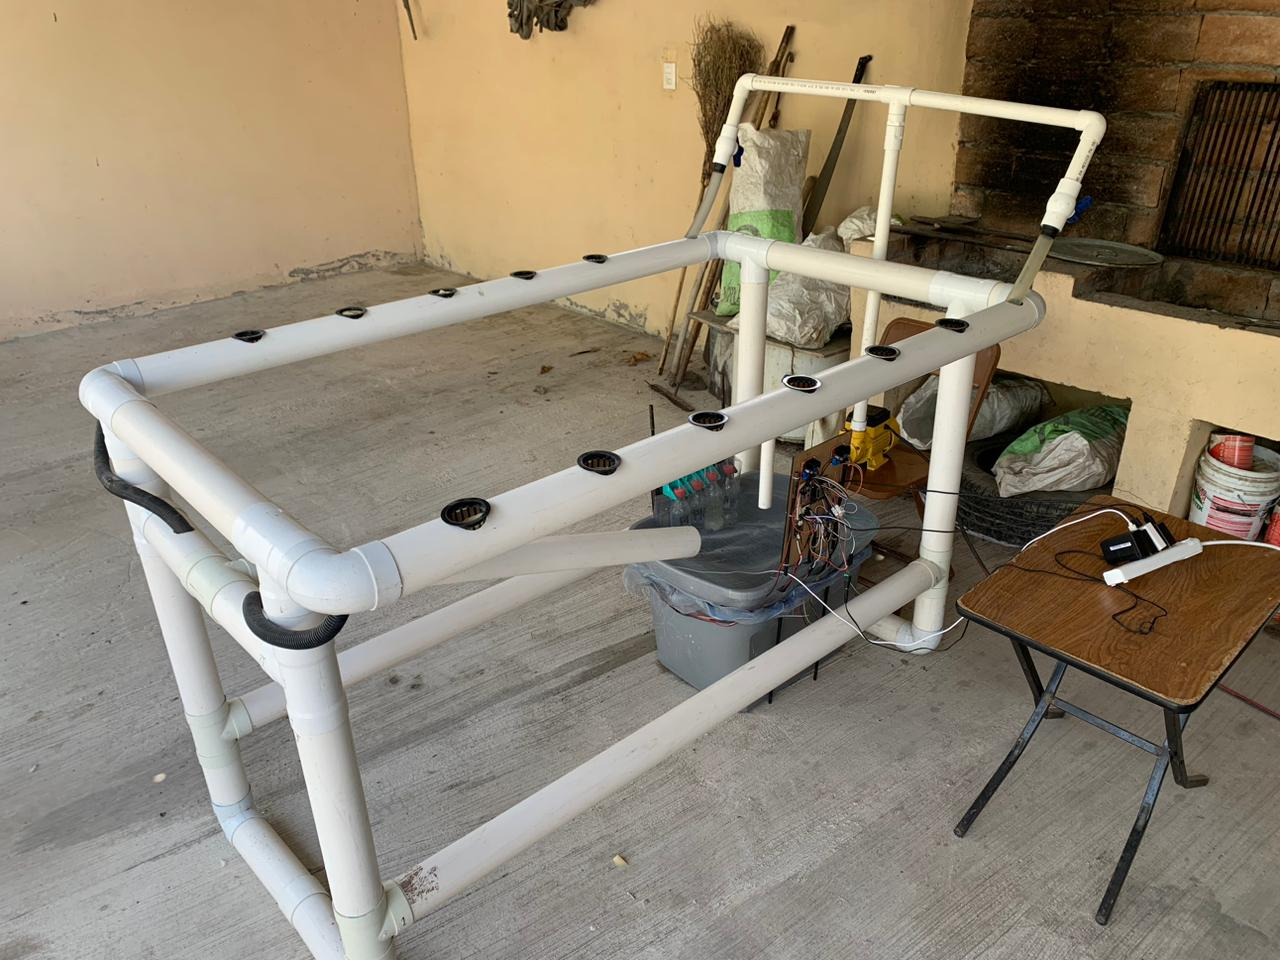
\includegraphics[scale=0.27]{imgs/dosCanales.jpg} \\
    \caption{Sistema hidropónico DFT propuesto de 2 canales. }\label{sistema8_2}
\end{figure}



\section{Pruebas funcionales del circuito de control}
El circuito de control está integrado por un microcontrolador ESP32, 4 bombas peristálticas y 4 sensores. Estos componentes están montados en una placa de acrílico. En la figura \ref{Peris}, se muestran las bombas peristálticas que fueron sujetadas por medio de soportes diseñados e impresos con filamento PLA. También se muestran los contenedores de 250 mililitros, los cuales contienen las siguientes sustancias: una solución alcalina con un pH de 10, una solución ácida con un pH de 4, un concentrado de nutrientes para el sistema y un último recipiente con agua.
 \begin{figure}[H]
\centering
         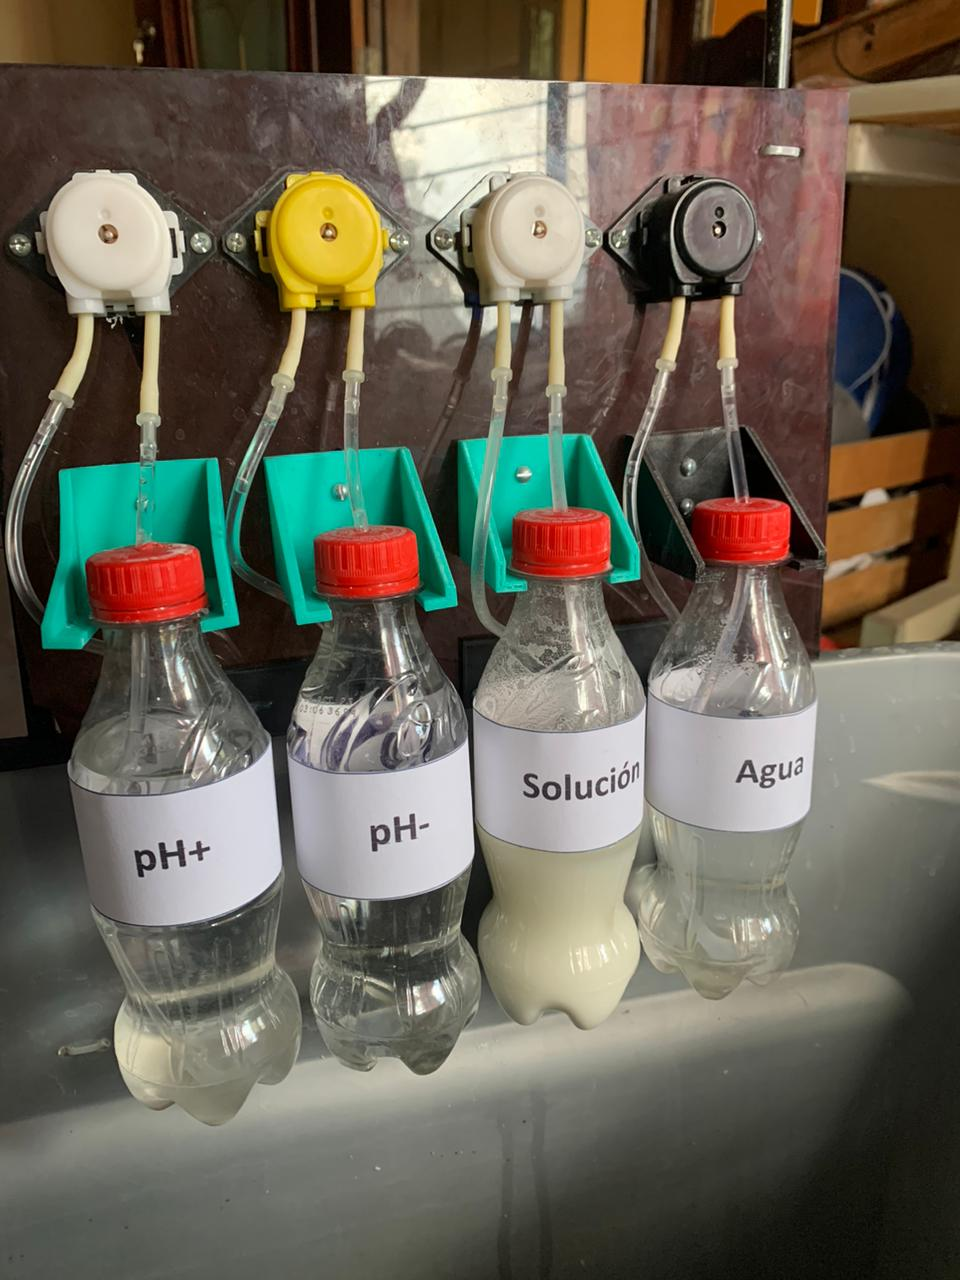
\includegraphics[scale=0.23]{imgs/perisss.jpg} \\
    \caption{Colocación de bombas peristálticas. }\label{Peris}
\end{figure}

En la figura \ref{flotador} se observan los sensores que contienen el sistema que son introducidos directamente en la solución nutritiva mediante una estructura de acrílico y flotadores que evitan que los sensores toquen el fondo del tanque y choquen con la minilavadora que se encarga del mezclado y oxigenación de la solución nutritiva.
 \begin{figure}[H]
\centering
         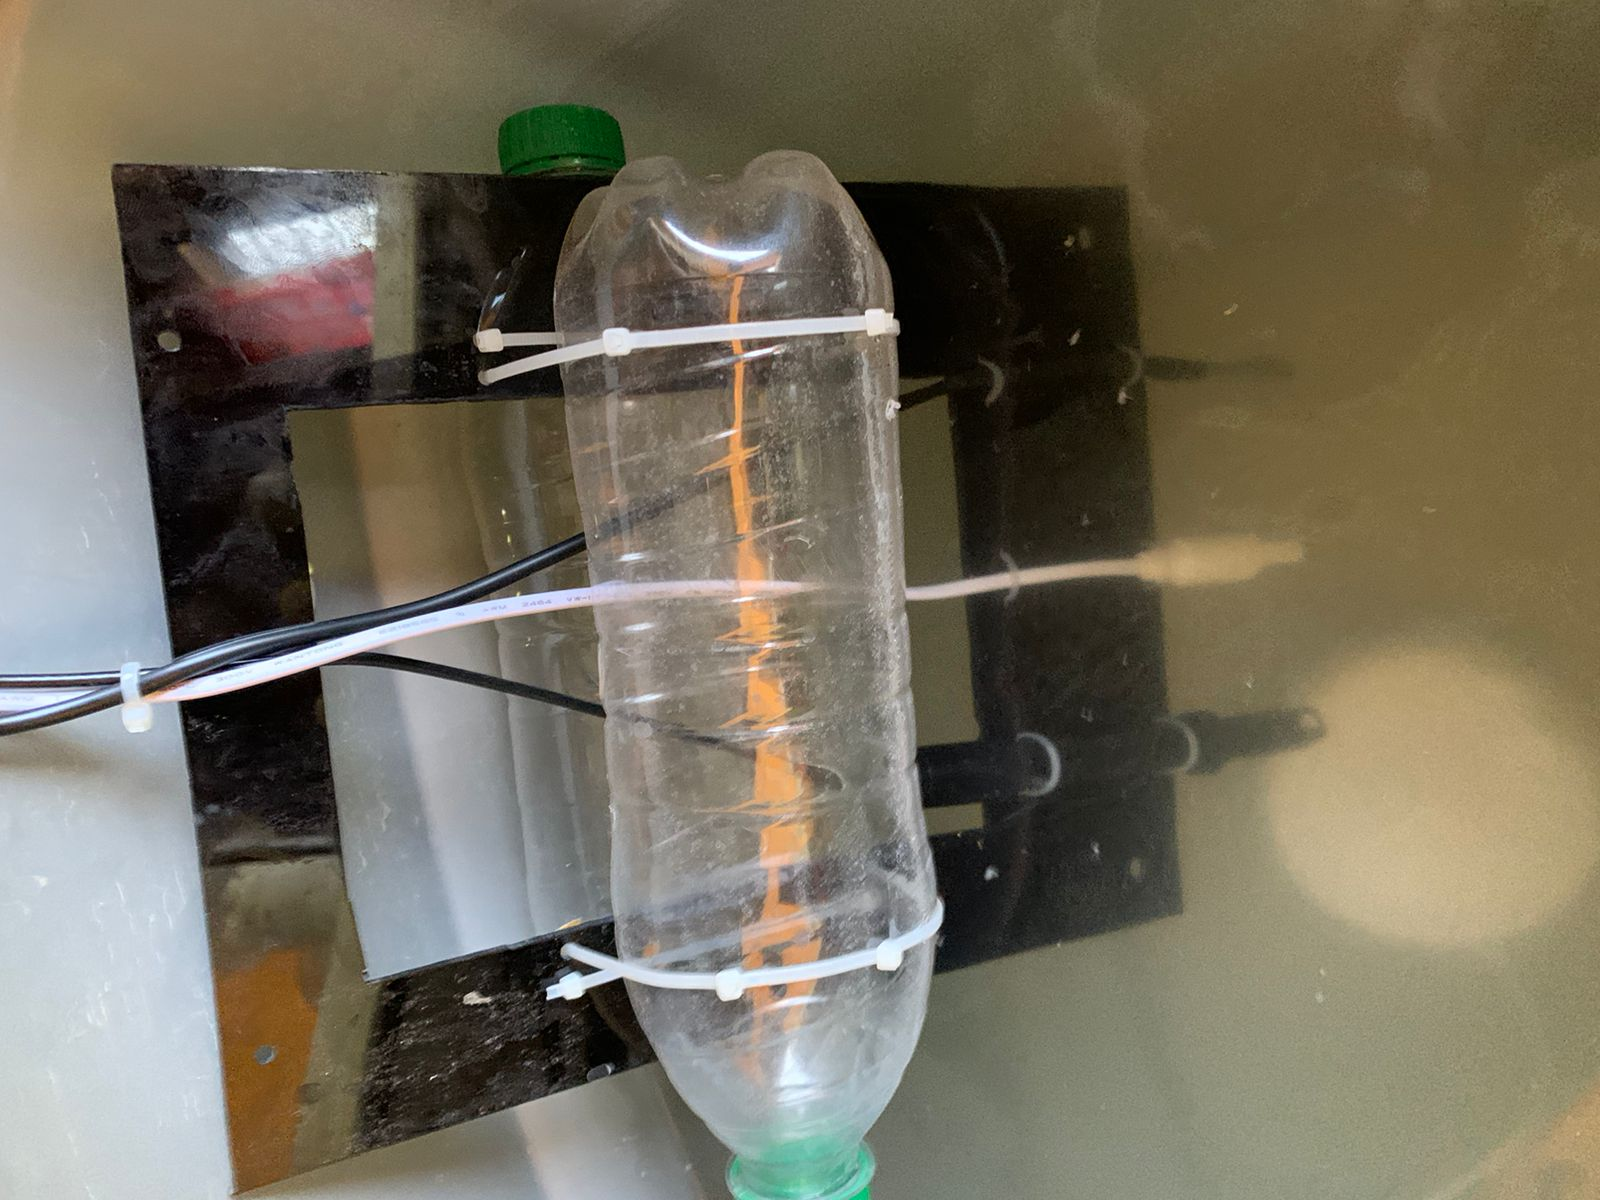
\includegraphics[scale=0.15]{imgs/flotador.jpg} \\
    \caption{Sensores con flotadores. }\label{flotador}
\end{figure}
La integración de todos los componentes del circuito de control en el tanque se muestran en la figura \ref{completo}. 
 \begin{figure}[H]
\centering
         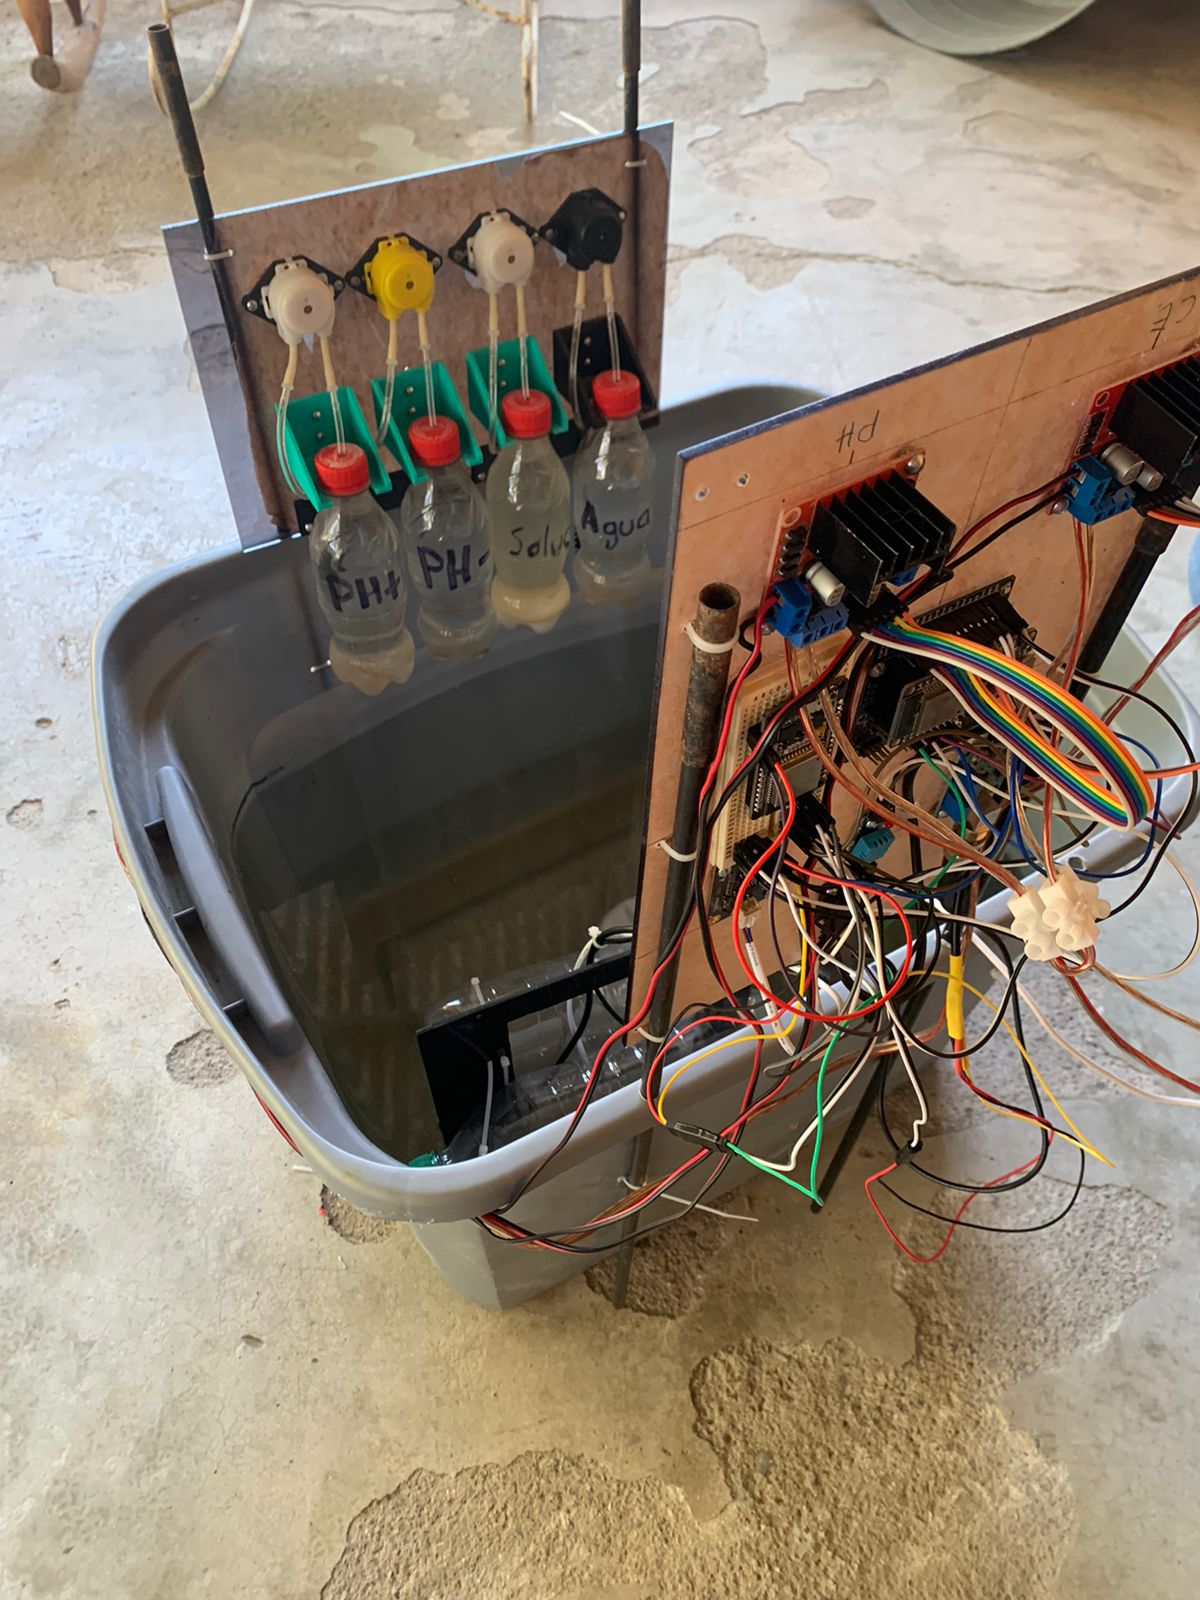
\includegraphics[scale=0.15]{imgs/circuitoCompleto.jpg} \\
    \caption{Componentes del circuito de control en el tanque. }\label{completo}
\end{figure}

\section{Control de dosificación de nutrientes}
\subsection{Simulación de la curva de control}
Para la implementación del controlador, primeramente se realizó una simulación de curva de control para la comparación de los datos de salida con la salida real en el sistema.  Para ello, se utilizó el lenguaje de programación Python y mediante funciones de la biblioteca \textit{scikit-fuzzy} se definieron funciones de membresía para los valores lingüísticos de entrada establecidos en el apartado \textit{ 4.4. Control difuso para la dosificación de nutrientes}. Estos términos son utilizados de dos formas: para la conductividad eléctrica en valores de error entre [-4000,4000] y de pH con valores de error entre [-14,14]. La salida del porcentaje de PWM es la misma para las dos situaciones, con una escala de porcentaje de [-100,100]. Como método de defusificación se utiliza el método del centroide y se despliega la curva de control utilizando funciones de la biblioteca \textit{matplotlib}. Las curvas de control en el caso del pH se muestran en la figura \ref{ph2} y la curva de control para la CE en la figura \ref{conduc2}.
\begin{figure}[H]
\centering
         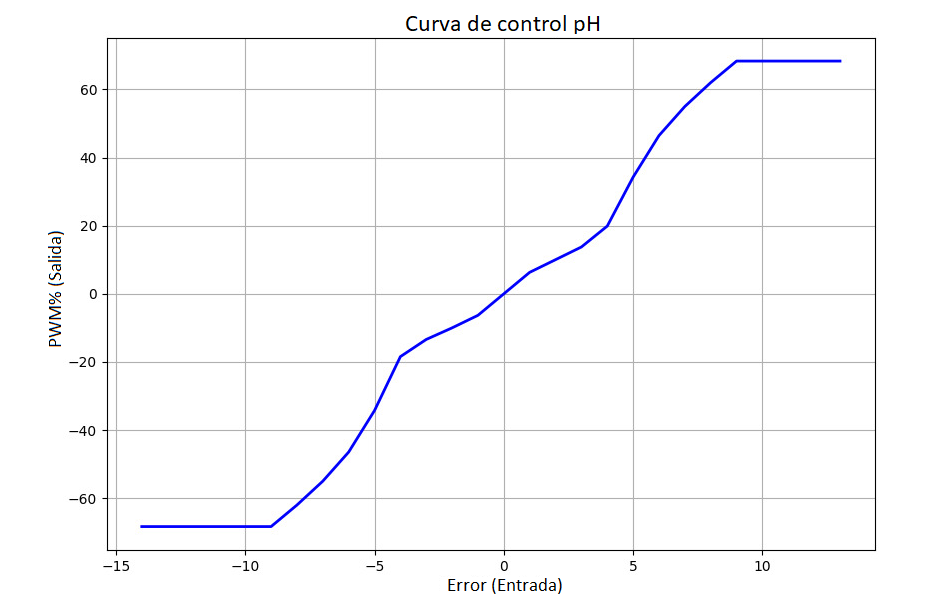
\includegraphics[scale=0.6]{imgs/CurvaPH_Esp.png} \\
    \caption{Curva de control para las bombas peristálticas que proveen las sustancias alcalina y ácida.}\label{ph2}
\end{figure}
\begin{figure}[H]
\centering
         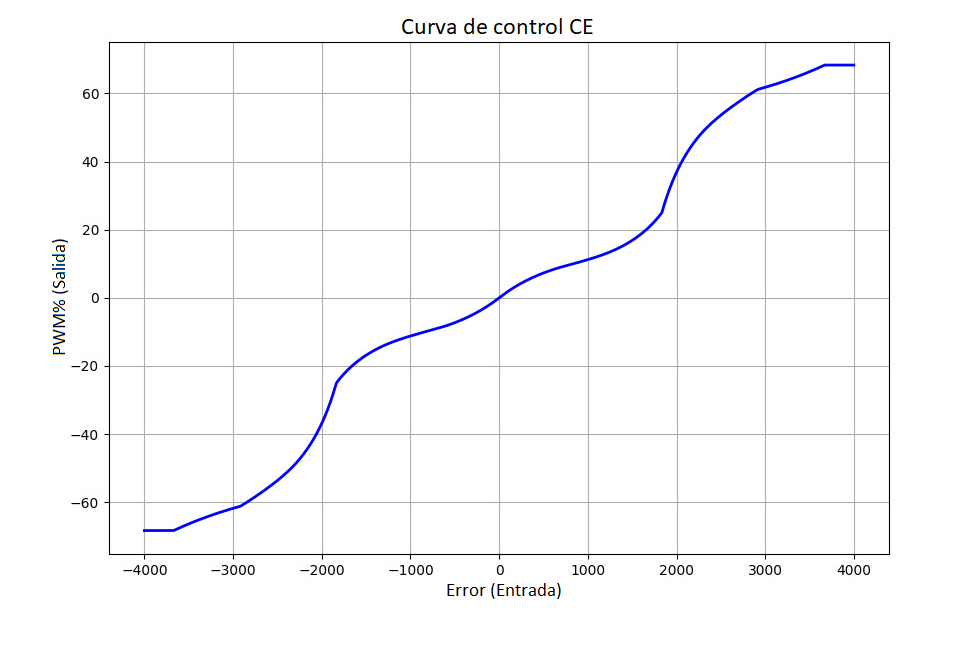
\includegraphics[scale=0.6]{imgs/CurvaCE_Esp.png} \\
    \caption{Curva de control para las bombas peristálticas del suministro del concentrado de solución nutritiva y agua.}\label{conduc2}
\end{figure}

\subsection{Implementación del controlador difuso}
%%%%%%%%%%%%%%%%%%%%%%%PH-----------%%%%%%%%%%%%%%%%%%%%%%%%%%%%%%%%
Para la programación del algoritmo del control difuso en el microcontrolador ESP32 se utilizó el entorno de desarrollo Arduino. El diagrama de flujo del algoritmo programado se puede observar en la figura \ref{flujo}.

\begin{figure}[H]
\centering
         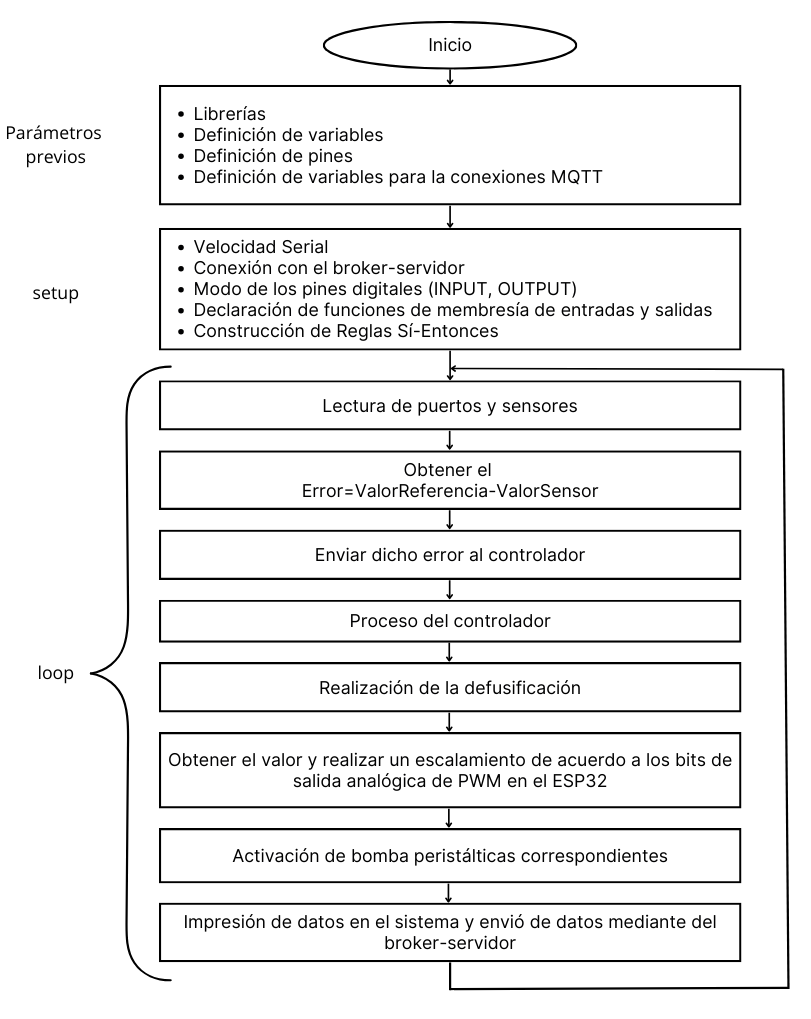
\includegraphics[scale=0.68]{imgs/Flujo (4).png} \\
    \caption{Diagrama de flujo del algoritmo de control difuso.}\label{flujo}
\end{figure}

Partiendo de la creación del algoritmo se generaron 4 casos específicos para las pruebas del controlador, que se describen a continuación. 

\subsubsection{Caso 1: Solución nutritiva con pH ácido}

En este caso, dentro del taque se realizó una disminución en el pH de la solución nutritiva llevándolo a un valor inicial cercano a 4. Como puede observarse en la gráfica superior de la figura \ref{PHMenos}, entre las muestras 18 y 32 el controlador realiza maniobras dentro del proceso en el ESP32 enviando información de porcentaje de PWM necesario para el control, como puede observarse en la gráfica central de la figura \ref{PHMenos}. Durante este proceso se puede observar que el controlador mantiene el valor de pH cerca del valor de referencia neutro de 7. Al mismo tiempo, en la gráfica inferior de la figura \ref{PHMenos} se muestra el valor de porcentaje de PWM en con una escala de voltaje entre 0 y 12 V.
\begin{figure}[H]
\centering
         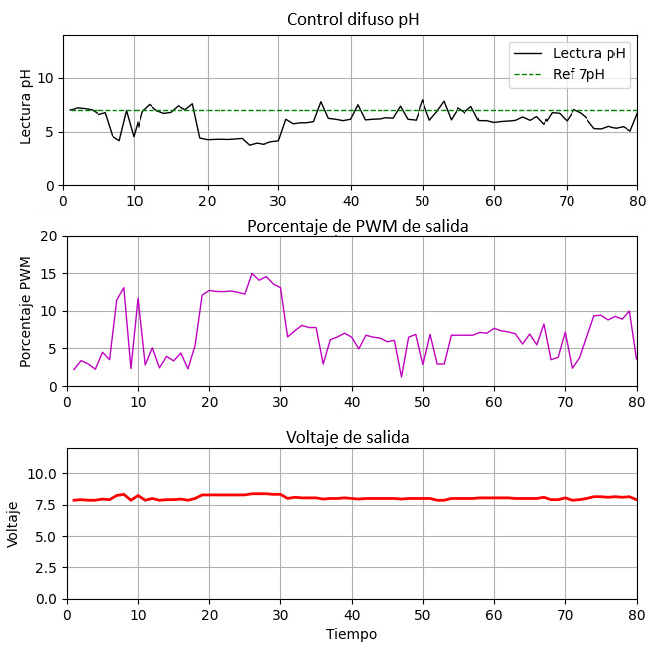
\includegraphics[scale=0.85]{imgs/phMenos.png} \\
    \caption{Señales obtenidas para el caso en el que se parte de una solución nutritiva con pH alcalino. En la gráfica superior se muestran los valores de lectura obtenidos del sensor de pH; En la gráfica central se muestran los valores de salida del controlador sobre el porcentaje de PWM; En la gráfica inferior se muestran los valores de voltaje de alimentación de las bombas peristálticas.}\label{PHMenos}
\end{figure}

%%%%%%%%%%%%%%%%%%%%%%%%%%%%%%%%%%%%%%%%%%%%%%%%%%%%%%%
%%%%%%%%%%%%%%%%%%%%%%%PH++++++++++++++%%%%%%%%%%%%%%%%%%%%%%%%%%%%%%%%
\newpage
\subsubsection{Caso 2: Solución nutritiva con pH alcalino}

En este caso se partió de un valor de pH cercano a 10, como se muestra en la gráfica superior de la figura \ref{PHMas}. Al empezar a funcionar, el controlador envía el porcentaje de PWM adecuado para disminuir el pH en la solución nutritiva, como se muestra en la gráfica central de la figura \ref{PHMas}. Durante el proceso el valor de pH se mantiene en el valor de referencia neutro de 7. En la gráfica inferior de la figura \ref{PHMas} se muestran las variaciones de voltaje ocurridas durante el control del pH.
\begin{figure}[H]
\centering
         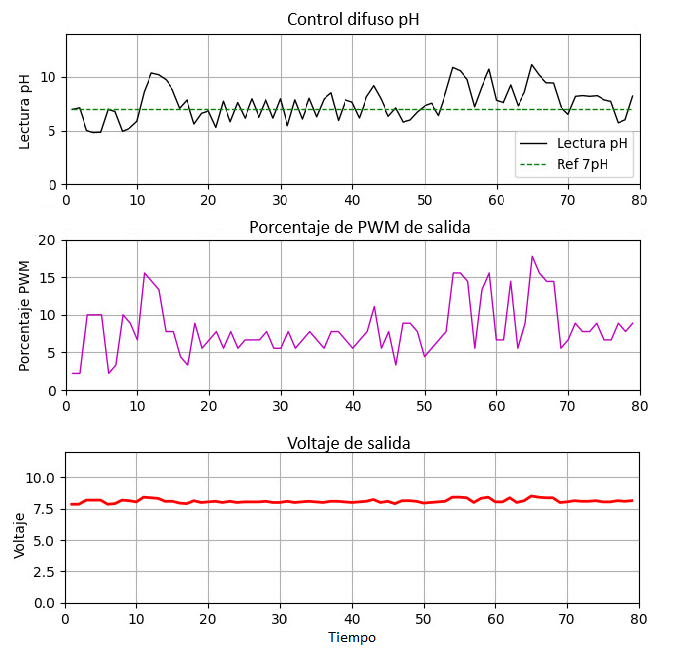
\includegraphics[scale=0.85]{imgs/phMas.png} \\
    \caption{Señales obtenidas para el caso en el que se parte de una solución nutritiva con pH alcalino. En la gráfica superior se muestran las lecturas obtenidas del sensor de pH; En la gráfica central se muestran los valores de salida del controlador sobre el porcentaje de PWM; En la gráfica inferior se muestran los valores de voltaje de alimentación de las bombas peristálticas.}\label{PHMas}
\end{figure}
%%%%%%%%%%%%%%%%%%%%%%%%%%%%%%%%%%%%%%%%%%%%%%%%%%%%%%%
%%%%%%%%%%%%%%%%%%%%%%%SolucionALTA++++++++++%%%%%%%%%%%%%%%%%%%%%%%%%%%%%%%%
\subsubsection{Caso 3: Solución nutritiva con bajo contenido de minerales}

Para el tercer caso se parte de una solución nutritiva con un nivel bajo de minerales y por lo tanto con una CE menor, con un valor inicial de alrededor de $450 \mu s/cm$, como se muestra en la gráfica superior de la figura \ref{CEMenos}. La gráfica central de la figura \ref{CEMenos} muestra el porcentaje de PWM generado por el controlador para aumentar el voltaje de alimentación de las bombas, mostrado en la gráfica inferior de la figura \ref{CEMenos}. El concentrado de minerales a usar debe ser preparado con antelación. La relación usada en esta preparación fue de 2 ml de minerales por cada litro de agua. 
\begin{figure}[H]
\centering
         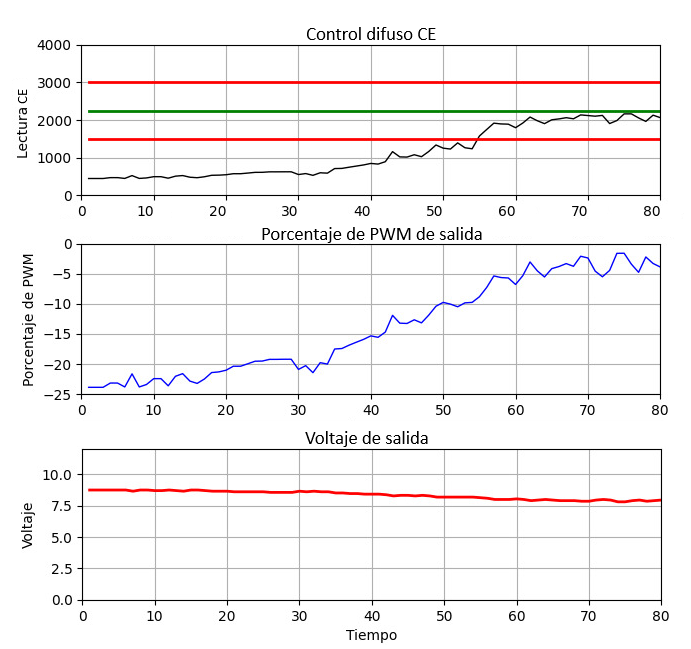
\includegraphics[scale=0.75]{imgs/CEMenos.png} \\
    \caption{Señales obtenidas para el caso en el que se parte de una solución nutritiva con bajo contenido de minerales. En la gráfica superior se muestran los valores de lectura obtenidos del sensor de CE; En la gráfica central se muestran los valores de salida del controlador sobre el porcentaje de PWM; En la gráfica inferior se muestran los valores de voltaje de salida hacia las bombas peristálticas.}\label{CEMenos}
\end{figure}
%%%%%%%%%%%%%%%%%%%%%%%%%%%%%%%%%%%%%%%%%%%%%%%%%%%%%%%
%%%%%%%%%%%%%%%%%%%%%%%Solucion baja---------------%%%%%%%%%%%%%%%%%%%%%%%%%%%%%%%%
\subsubsection{Caso 4: Solución nutritiva con alta concentración de minerales}

En este último caso, a una solución nutritiva con valor de CE por debajo del límite inferior, se le agregó aproximadamente $\frac{1}{4}$ de taza de sal, ya con el sistema funcionando, para incrementar el valor de CE de alrededor de $1200 \mu s/cm$ a $4200 \mu s/cm$, como se muestra en la gráfica superior de la figura \ref{CEMas}. A diferencia del caso de donde se partió de una solución con baja concentración de sales, en este caso el controlador tardó más muestras en alcanzar el rango deseado después de haber incrementado la CE debido a que fue necesario utilizar más agua como disolvente para lograr el objetivo de control, llegando a los límites de error que pueden existir en el universo empleado. La gráfica central de la figura \ref{CEMas} muestra el porcentaje de PWM enviado por el controlador, mientras que la gráfica inferior de la figura \ref{CEMas} muestra el voltaje enviado a las bombas peristálticas correspondientes.

\begin{figure}[H]
\centering
         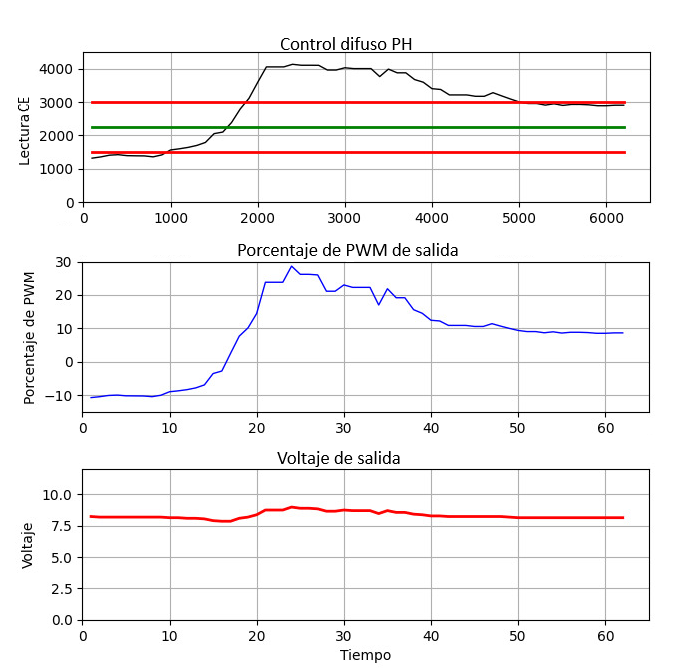
\includegraphics[scale=0.75]{imgs/CEMas.png} \\
    \caption{Señales obtenidas para el caso en el que se parte de una solución nutritiva con alta concentración de minerales. En la gráfica superior se muestran los valores de lectura obtenidos del sensor de CE; En la gráfica central se muestra la salida del controlador sobre el porcentaje de PWM; En la gráfica inferior se muestra el voltaje de salida hacia las bombas peristálticas.}\label{CEMas}
\end{figure}

%%%%%%%%%%%%%%%%%%%%%%%%%%%%%%%%%%%%%%%%%%%%%%%%%%%%%%%
\section{Monitoreo de variables}

Para poder monitorear las variables a distancia mediante el protocolo MQTT, fue necesario configurar un \textit{broker} (figura \ref{broker}). 
Por medio del \textit{broker}, se enlazan las interfaces mediante una suscripción a un tópico, y el \textit{broker} se encarga de distribuir la información recibida entre todos los componentes que están suscritos a dicho tópico. El microcontrolador ESP32 se encarga de obtener las lecturas de los sensores, y publicarlas en la plataforma Node-Red para su posterior distribución. La aplicación móvil recibe las notificaciones de las lecturas publicadas, ya que es un dispositivo que también está suscrito a dichos tópicos. En las figuras \ref{servidor} y \ref{app}, se muestra el estado de las interfaces cuando ya están suscritas a dichos tópicos y cuando el sistema ya está en operación. Las interfaces despliegan gráficas que dan evidencia del comportamiento de los sensores en función del tiempo.   
%Para ello se enlazan cada una de las interfaces al suscribirse al \textit{broker} y este mismo distribuye la información publicada por el ESP32 hacia el servidor Node-Red y la aplicación móvil, como se observa en las figuras \ref{servidor} y \ref{app} respectivamente. La información de los parámetros se obtienen de los sensores que se encuentran en la solución nutritiva, dichos parámetros son: la temperatura, la humedad, la conductividad eléctrica y el pH de la solución.

 \begin{figure}[H]
\centering
         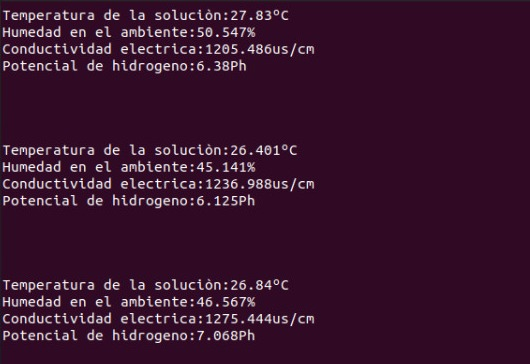
\includegraphics[scale=0.7]{imgs/broker.jpeg} \\
    \caption{Publicación de datos en el \textit{broker} mosquitto.}\label{broker}
\end{figure}
\begin{figure}[H]
\centering
         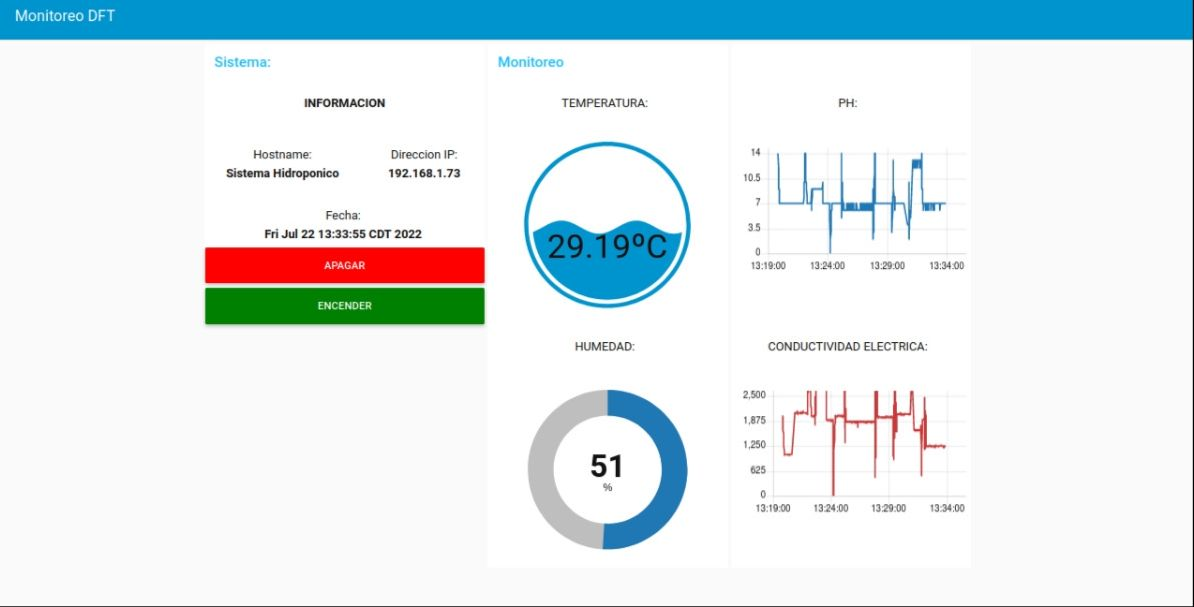
\includegraphics[scale=0.4]{imgs/servidor1.jpeg} \\
    \caption{Visualización de las lecturas obtenidas mediante la interfaz web proporcionada por la plataforma Node-red.} \label{servidor}
\end{figure}

\begin{figure}[H]
\centering
         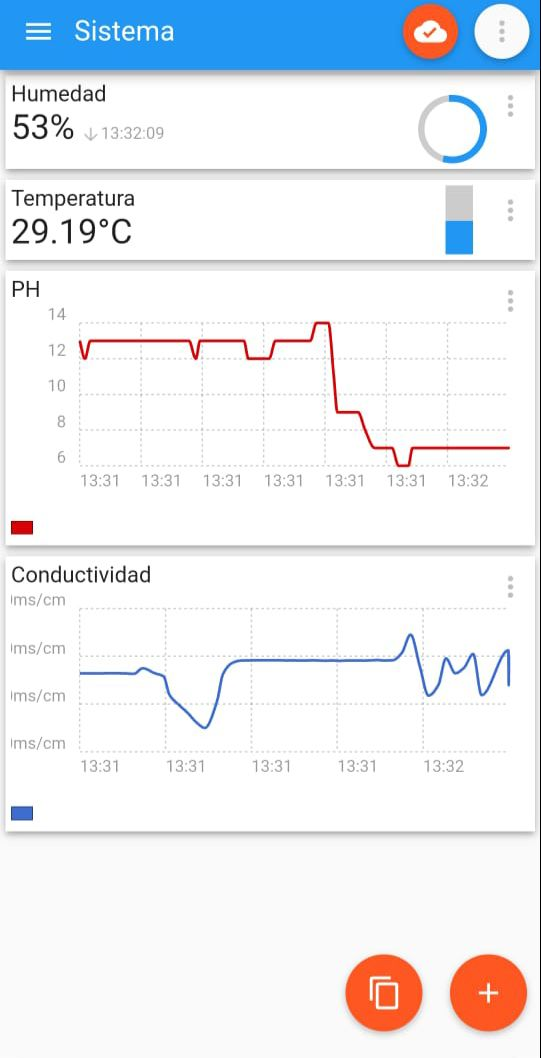
\includegraphics[scale=0.5]{imgs/app1.jpeg} \\
    \caption{Visualización de las lecturas obtenidas mediante la aplicación móvil vinculada con la plataforma Node-Red.} \label{app}
\end{figure}



\section{Monitoreo de germinación}

\subsection{Visión por computadora}
Para el monitoreo de germinación de las plantas se programó un \textit{script} en el lenguaje de programación Python con las bibliotecas de OpenCV, el cual realiza la captura de video en tiempo real utilizando una cámara web, que se encuentra dirigida hacia los semilleros. En este \textit{script} se implementa un método de segmentación, donde sobre cada cuadro del video se realiza un cambio del espacio de colores BGR a HSV. Enseguida se genera una máscara binaria correspondiente a los tonos en verde observado en el semillero con la cual se segmentan las zonas correspondientes a las plantas. Al realizar capturas cada día y compararlas se puede observar el crecimiento de las plantas. Los resultados de este proceso se puede observar en las figuras \ref{cam}, \ref{foto} y \ref{segmentacion}.

\begin{figure}[H]
\centering
         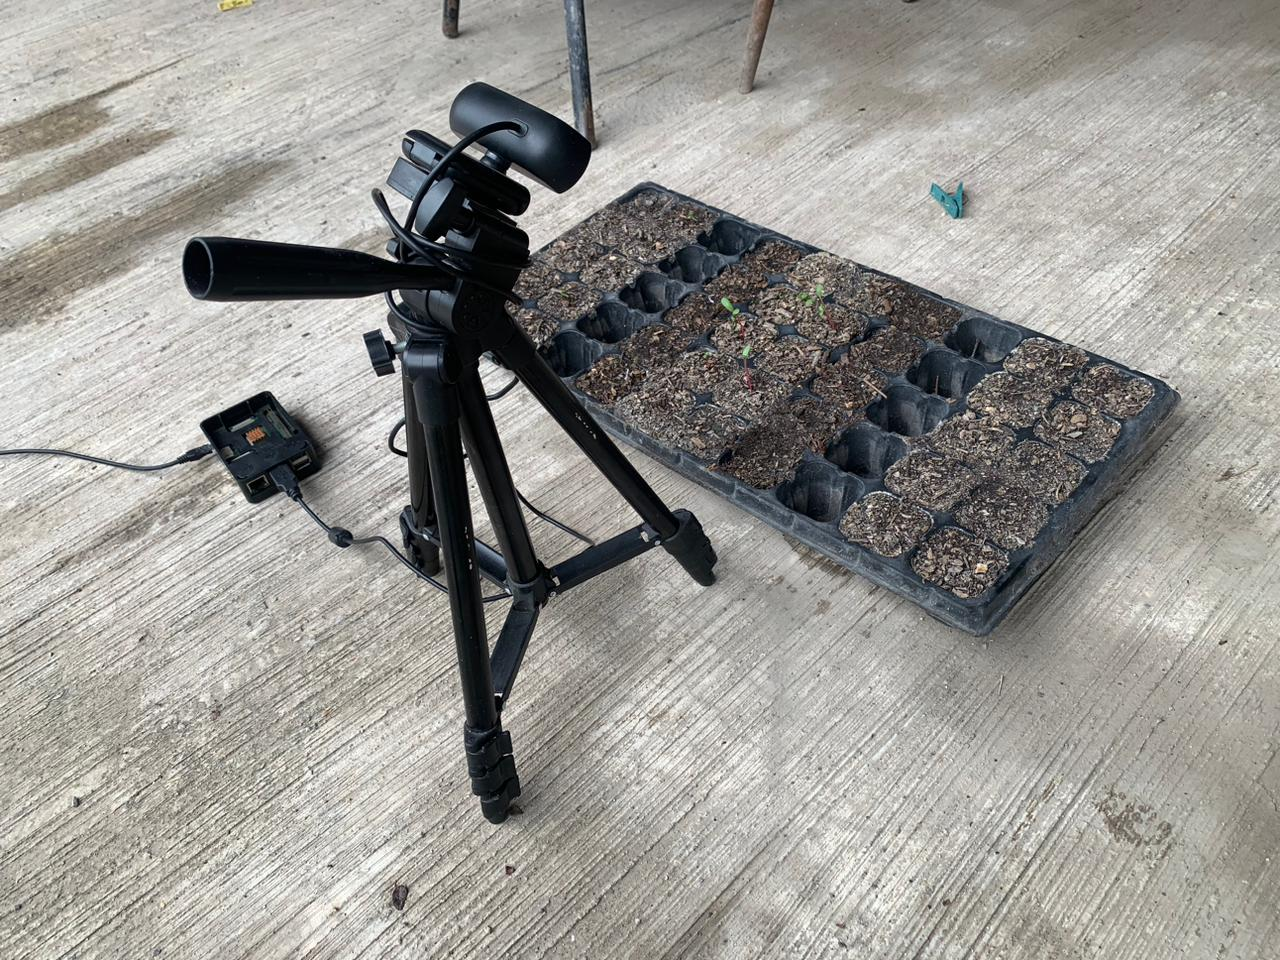
\includegraphics[scale=0.2]{imgs/Camara.jpg}
    \caption{Colocación de la cámara en los semilleros.}\label{cam}
\end{figure}

\begin{figure}[H]
\centering
         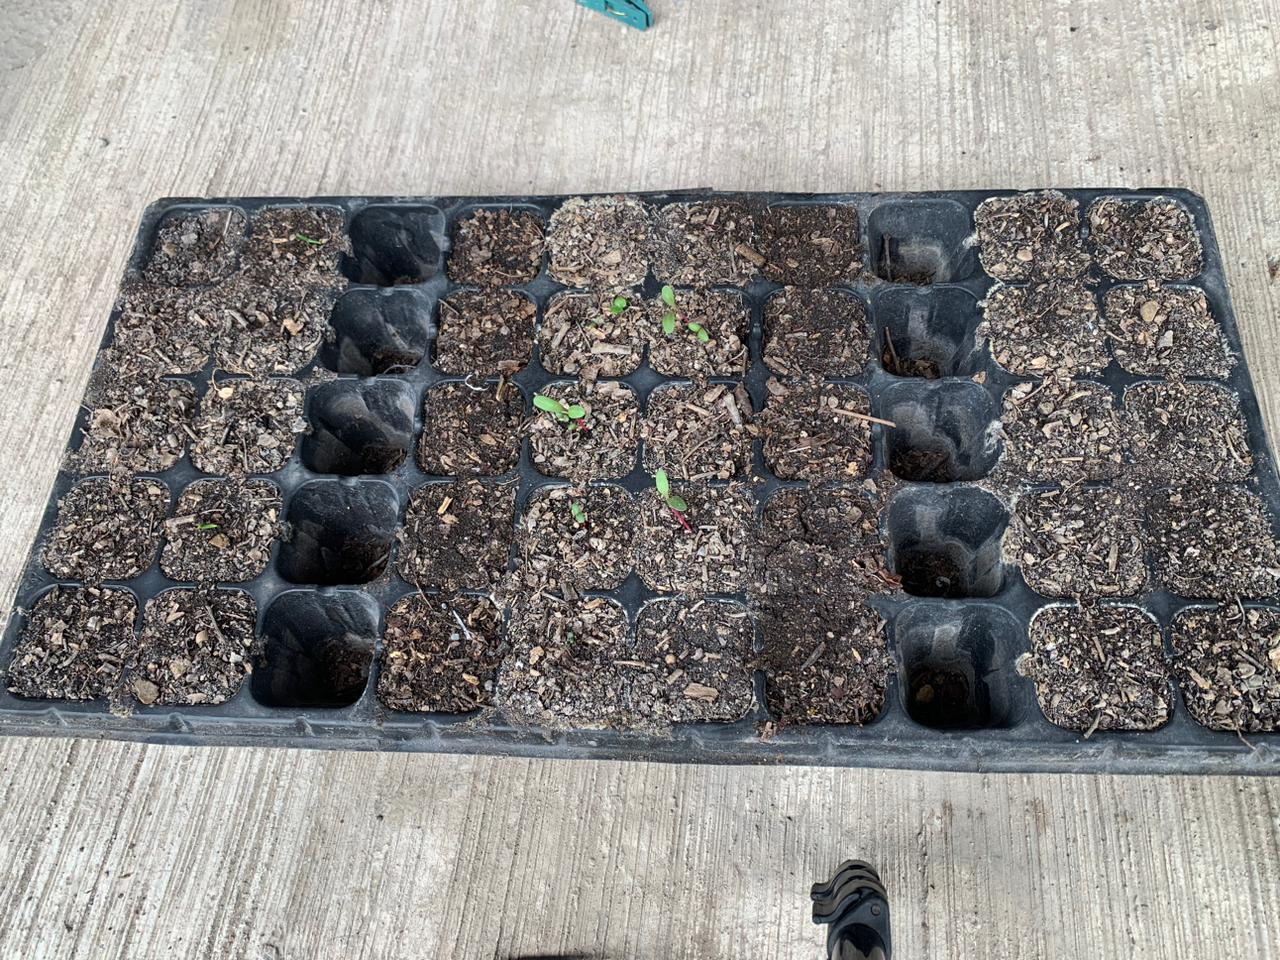
\includegraphics[scale=0.2]{imgs/fotoCamara.jpg}
    \caption{Fotografía de los semilleros.}\label{foto}
\end{figure}

\begin{figure}[H]
\centering
         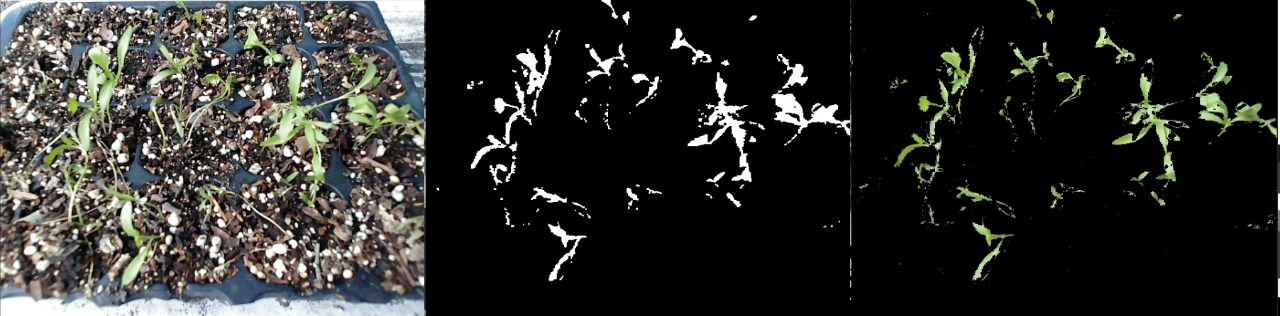
\includegraphics[scale=0.35]{imgs/germinacion.jpeg}
    \caption{Segmentación de las plantas germinadas.}\label{segmentacion}
\end{figure}

\section{Discusión}
La implementación de algoritmos de control difuso en los sistemas hidropónicos es una estrategia que permite controlar los nutrientes de importancia en el crecimiento de las plantas, buscando mejorar la producción.

Sin embargo, es importante señalar algunos desafíos asociados con la implementación del control difuso en sistemas hidropónicos. Por un lado, se debe tener conocimientos técnicos acerca del tema para la configuración inicial de los conjuntos de reglas difusas y los parámetros del controlador. Además, la precisión del control difuso puede depender en gran medida de la calidad y la confiabilidad de los sensores y actuadores utilizados.

Por otro lado, la utilización de un control difuso presenta un enfoque prometedor para maximizar la productividad de los cultivos. Si se implementa y ajusta correctamente, esta técnica puede contribuir significativamente al control automático de sistemas hidropónicos usados en agricultura. Sin embargo, se deben realizar más experimentos con otros tipos de sistemas de agricultura en interiores para comprobar su eficacia en estos casos.

\section{Análisis de costos del proyecto}
El análisis de costos del proyecto se llevó a cabo tomando los aspectos más importantes dentro del sistema, incluyendo los materiales de la estructura hidropónica y del circuito de control. Este análisis se basa en los precios obtenidos el día 5 de mayo del 2023 en pesos mexicanos. El tiempo de construcción del sistema, ya teniendo todos los componentes y herramientas fue de alrededor de 5 días.

\textbf{Sistema hidropónico DFT de 8 canales}

\begin{table}[H]
\centering
\caption{Análisis de costos del sistema a 8 canales.} 
\begin{tabular}{|p{4.7cm}|p{1.85cm}|p{2.5cm}|p{1.8cm}|p{2.2cm}|}
\hline
           \textbf{Material} & \textbf{Cantidad} & \textbf{Unidad} & \textbf{Costo unitario} & \textbf{Costo total} \\
\noalign{\hrule height 2pt}

        Tubo PVC de 3 pulgadas &  22  & Metros & \$29.00& \$638.00  \\
        \hline
        Codo PVC de 3 pulgadas &  8 & Pieza & \$15.00& \$120.00\\
       \hline
        T PVC de 3 pulgadas &  23 & Pieza & \$25.00& \$575.00\\
     \hline
      Tubo hidráulico de 1 pulgadas &   4.5 & Metros & \$30.00& \$135.00  \\
        \hline
        Codo de 1 pulgadas &  4 & Pieza & \$10.00& \$40.00\\
       \hline
        T de 1 pulgadas &  8 & Pieza & \$10.00& \$80.00\\
         \hline
     Cople Tipo Hembra 1 pulgada & 1   & Pieza & \$10.00& \$10.00 \\
          \hline
     Cople Tipo Macho 1 pulgada & 3  & Pieza & \$10.00& \$30.00\\
           \hline
     Llave de paso 1 pulgada & 9  & Pieza & \$65.00& \$585.00 \\
            \hline
     Tubo cristalino 1 pulgada & 3  & Metros & \$40.00& \$120.00 \\
            \hline
     Pegamento para PVC & 2  & Pieza & \$190.00& \$280.00 \\
            \hline
     Canastilla de 2 pulgadas & 44  & Pieza & \$9.00& \$396.00 \\
            \hline
      &   &  &  \textbf{Total :}& \$3009.00 \\
            \hline

       

\end{tabular}
\label{tab:t3}
\end{table}

\newpage
\textbf{Sistema hidropónico DFT de 2 canales.}

\begin{table}[H]
\centering
\caption{Análisis de costos del sistema a 2 canales.} 
\begin{tabular}{|p{4.7cm}|p{1.85cm}|p{2.5cm}|p{1.8cm}|p{2.2cm}|}
\hline
      \textbf{Material} & \textbf{Cantidad} & \textbf{Unidad} & \textbf{Costo unitario} & \textbf{Costo total} \\
\noalign{\hrule height 2pt}

        Tubo PVC de 3 pulgadas &  14  & Metros & \$29.00& \$406.00  \\
        \hline
        Codo PVC de 3 pulgadas &  8 & Pieza & \$15.00& \$120.00\\
       \hline
        T PVC de 3 pulgadas &  10 & Pieza & \$25.00& \$250.00\\
     \hline
      Tubo hidráulico de 1 pulgadas &   2.5 & Metros & \$30.00& \$75.00  \\
        \hline
        Codo de 1 pulgadas &  4 & Pieza & \$10.00& \$40.00\\
       \hline
        T de 1 pulgadas &  2 & Pieza & \$10.00& \$20.00\\
         \hline
     Cople Tipo Hembra 1 pulgada & 1   & Pieza & \$10.00& \$10.00 \\
          \hline
     Cople Tipo Macho 1 pulgada & 3  & Pieza & \$10.00& \$30.00\\
           \hline
     Llave de paso 1 pulgada & 3  & Pieza & \$65.00& \$185.00 \\
            \hline
     Tubo cristalino 1 pulgada & 1  & Metros & \$40.00& \$40.00 \\
            \hline
     Pegamento para PVC & 1  & Pieza & \$155.00& \$155.00 \\
            \hline
     Canastilla de 2 pulgadas & 11  & Pieza & \$9.00& \$99.00 \\
            \hline
      &   &  &  \textbf{Total :}& \$1430.00 \\
            \hline


\end{tabular}
\label{tab:t4_r}
\end{table}
\newpage
\textbf{Circuito de control}

\begin{table}[H]
\centering
\caption{Análisis de costos del circuito de control.} 
\begin{tabular}{|p{4.7cm}|p{1.85cm}|p{2.5cm}|p{1.8cm}|p{2.2cm}|}
\hline
                  \textbf{Material} & \textbf{Cantidad} & \textbf{Unidad} & \textbf{Costo unitario} & \textbf{Costo total} \\
\noalign{\hrule height 2pt}

        Microcontrolador ESP32 & 1   & Pieza & \$209.00& \$209.00  \\
        \hline
        Raspberry pi 3 b+ &  1 & Pieza & \$2045.00& \$2045.00\\
       \hline
     Sensor Dht11 &  1 & Pieza & \$65.00& \$65.00\\
     \hline
     Sensor PH-4502C & 1 & Pieza & \$535.00& \$535.00\\
     \hline
     Sensor TDS meter v1 &  1& Pieza & \$630.00& \$630.00\\
      \hline
     Sensor DS18B20 &   1 & Pieza & \$58.00& \$58.00\\
         \hline
     Driver Puente H L298N & 2   & Pieza & \$75.00& \$150.00 \\
          \hline
     Modulo relé de 2 canales & 1  & Pieza & \$150.00& \$150.00\\
           \hline
     Bombas peristálticas  & 4  & Pieza & \$122.00& \$488.00 \\
            \hline
             Bomba periférica 1/2 Hp & 1  & Pieza & \$436.00& \$436.00 \\
            \hline
             Minilavadora & 4  & Pieza & \$205.00& \$205.00 \\
            \hline
      &   &  &  \textbf{Total :}& \$4971.00 \\
            \hline

       

\end{tabular}
\label{tab:t5}
\end{table}


%%%%%%%%%%%%%%%%%%%%%%%%%%%%%%%%%%%%%%%%%%%%%%%%%%%%%%%%
%%%%%%%%%%%%%%%%%%%%%%%%%%%%%%%%%%%%%%%%%%%%%%%%%%%%%%%%%%%%%%%%%%%%%%%%%%%%%%%%%%%%%%%%%%%%%%%%%%%